\section{Appendix}

\subsection{MovieLens 1M: Detailed Exploratory Data Analysis}
\label{app:ml1m-eda}

This appendix presents the full exploratory data analysis of the MovieLens~1M dataset used in Regime~1 (\S\ref{sec:eval-movies}).
All statistics were computed from the original data files (\texttt{users.dat}, \texttt{ratings.dat}, \texttt{movies.dat}) after verifying referential integrity (zero orphan records).

\subsubsection{Dataset Overview}

Table~\ref{tab:ml1m-summary} summarizes the key statistics.

\begin{table}[h]
\centering
\caption{ML-1M dataset summary statistics.}
\label{tab:ml1m-summary}
\small
\begin{tabular}{@{}lr@{}}
\toprule
\textbf{Statistic} & \textbf{Value} \\
\midrule
Users & 6{,}040 \\
Movies & 3{,}883 \\
Ratings & 1{,}000{,}209 \\
Sparsity & 95.74\% \\
Rating scale & 1--5 (whole stars) \\
Mean rating & 3.582 ($\sigma=1.117$) \\
Timestamp range & Apr 2000 -- Feb 2003 \\
Months with activity & 35 \\
\midrule
\multicolumn{2}{@{}l}{\textit{Per-user ratings}} \\
\quad Mean / Median & 165.6 / 96 \\
\quad Min / Max & 20 / 2{,}314 \\
\quad Std & 192.7 \\
\midrule
\multicolumn{2}{@{}l}{\textit{Per-movie ratings}} \\
\quad Mean / Median & 269.9 / 124 \\
\quad Min / Max & 1 / 3{,}428 \\
\quad Std & 384.0 \\
\bottomrule
\end{tabular}
\end{table}


\subsubsection{Rating Distribution}

The rating distribution is left-skewed (Figure~\ref{fig:app-rating-dist}): 4-star ratings are most common (348{,}971; 34.9\%), followed by 3 stars (261{,}197; 26.1\%), 5 stars (226{,}310; 22.6\%), 2 stars (107{,}557; 10.8\%), and 1 star (56{,}174; 5.6\%).
The mean rating of 3.582 confirms an overall positive-skew consistent with prior work on self-selected rating systems.

\begin{figure}[h]
    \centering
    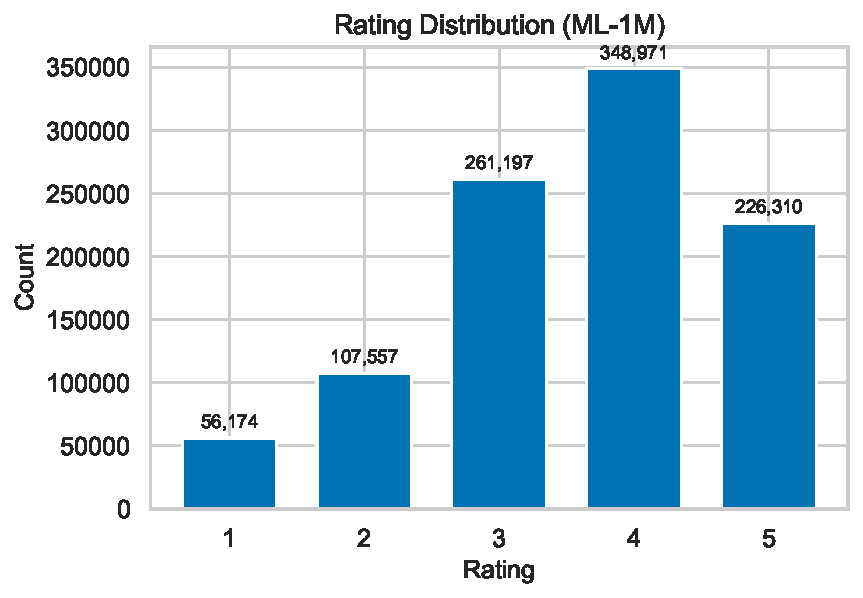
\includegraphics[width=0.6\columnwidth]{images/ml1m_rating_distribution.pdf}
    \caption{Overall rating distribution in ML-1M.}
    \label{fig:app-rating-dist}
\end{figure}


\subsubsection{User Demographics}
\label{app:demographics}

\paragraph{Gender.}
The dataset is 71.7\% male (4{,}331 users) and 28.3\% female (1{,}709 users), reflecting the demographics of early-2000s online movie communities.

\paragraph{Age.}
Figure~\ref{fig:app-demographics} shows the age distribution.
The 25--34 bracket is largest (2{,}096 users, 34.7\%), followed by 18--24 (1{,}103, 18.3\%) and 35--44 (1{,}193, 19.8\%).
Under-18 (222, 3.7\%) and 56+ (380, 6.3\%) are the smallest groups.

\paragraph{Occupation.}
The top five occupations are: college/grad student (759, 12.6\%), other/not specified (711, 11.8\%), executive/managerial (679, 11.2\%), academic/educator (528, 8.7\%), and technician/engineer (502, 8.3\%).
The rarest occupations are farmer (17 users, 0.3\%), tradesman/craftsman (70, 1.2\%), and unemployed (72, 1.2\%).

\begin{figure}[h]
    \centering
    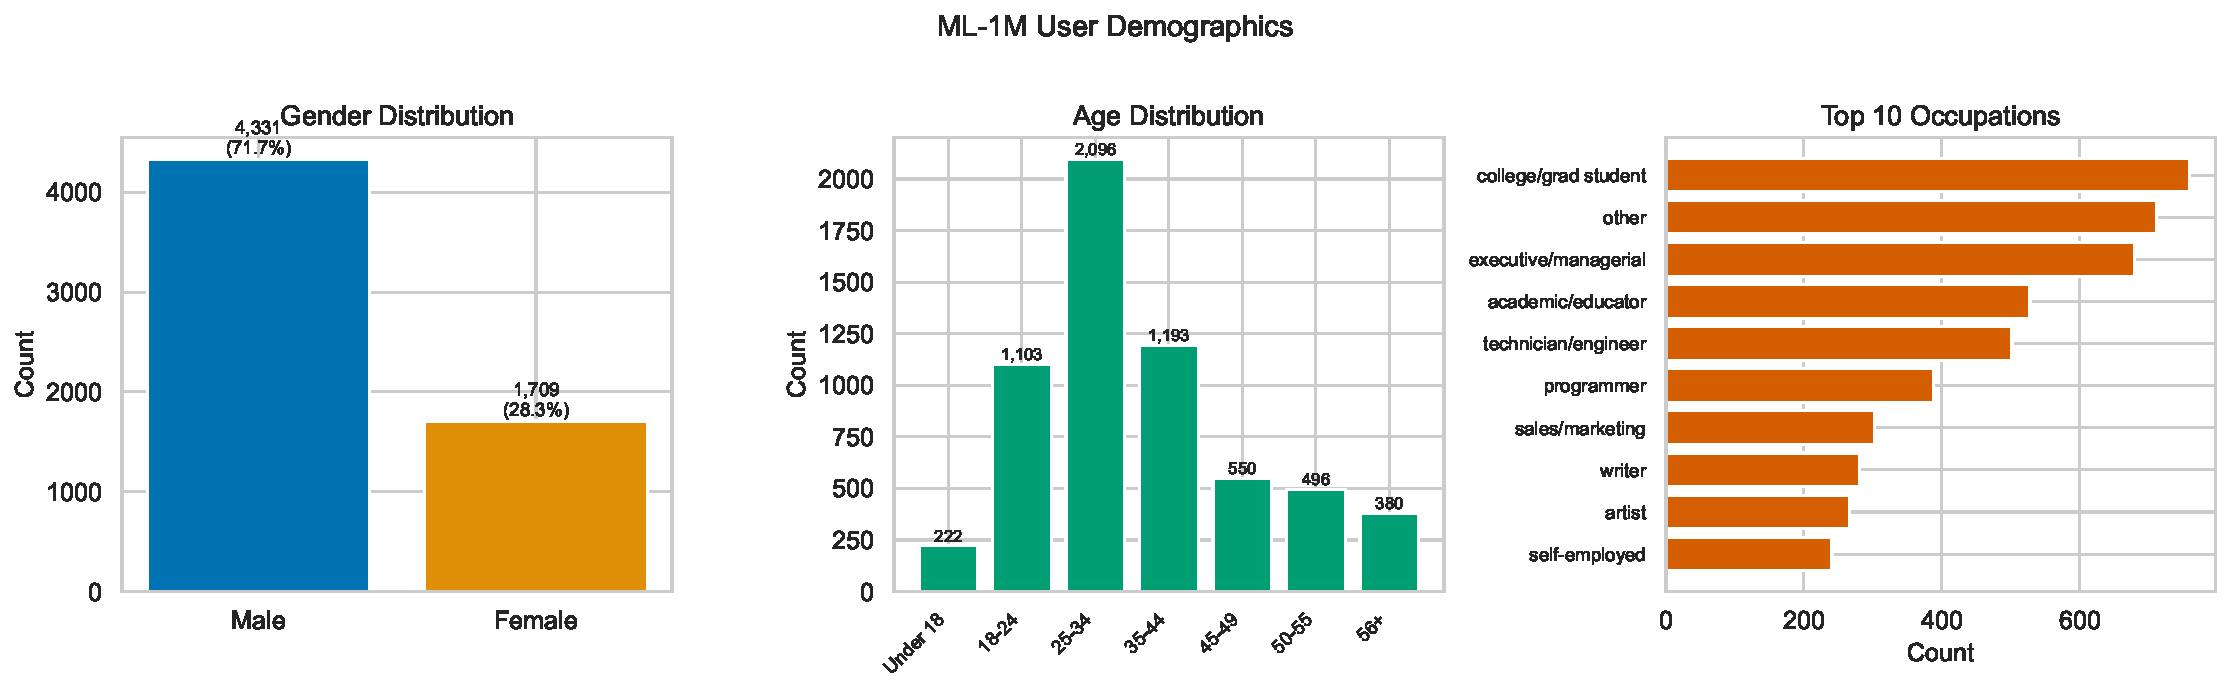
\includegraphics[width=\textwidth]{images/ml1m_demographics.pdf}
    \caption{User demographic distributions: gender, age, and top-10 occupations.}
    \label{fig:app-demographics}
\end{figure}


\subsubsection{Gender $\times$ Age Cross-Tabulation}

Table~\ref{tab:gender-age} and Figure~\ref{fig:app-gender-age} show the Gender$\times$Age cross-tabulation.
All 14 cells are non-empty; the smallest cell (Female Under~18) contains 78 users, confirming that Gender$\times$Age is a viable primary stratification axis.

\begin{table}[h]
\centering
\caption{Gender $\times$ Age cross-tabulation (user counts).}
\label{tab:gender-age}
\small
\begin{tabular}{@{}lrr@{}}
\toprule
\textbf{Age Group} & \textbf{Female} & \textbf{Male} \\
\midrule
Under 18 & 78 & 144 \\
18--24 & 298 & 805 \\
25--34 & 558 & 1{,}538 \\
35--44 & 338 & 855 \\
45--49 & 189 & 361 \\
50--55 & 146 & 350 \\
56+ & 102 & 278 \\
\midrule
\textbf{Total} & \textbf{1{,}709} & \textbf{4{,}331} \\
\bottomrule
\end{tabular}
\end{table}

\begin{figure}[h]
    \centering
    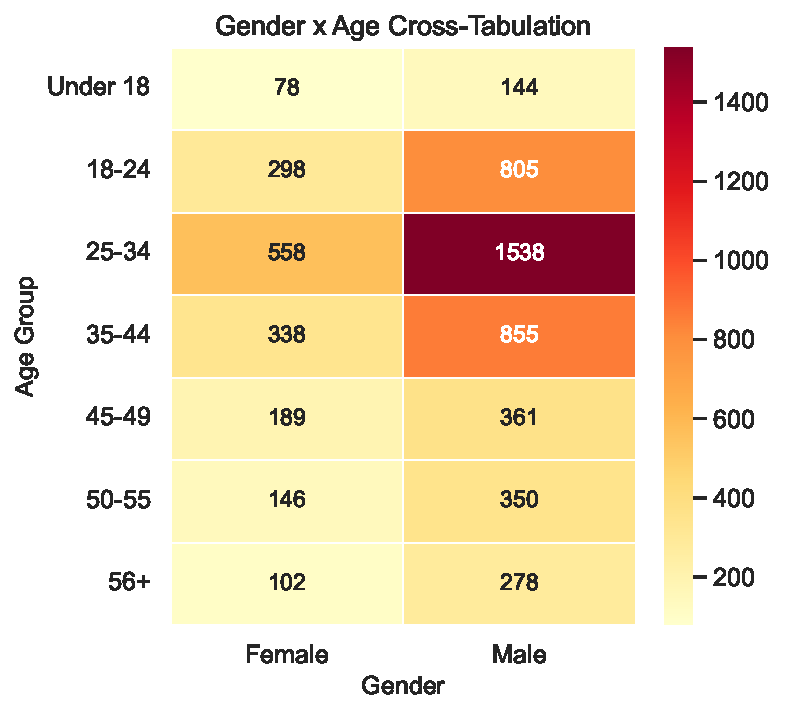
\includegraphics[width=0.5\columnwidth]{images/ml1m_gender_age_heatmap.pdf}
    \caption{Gender $\times$ Age heatmap showing user counts per cell.}
    \label{fig:app-gender-age}
\end{figure}


\subsubsection{Subgroup Sparsity Analysis}
\label{app:sparsity}

When all three demographic axes are combined (Gender$\times$Age$\times$Occupation), the 294 possible cells decompose as:

\begin{itemize}
    \item 53 empty cells (18.0\%)
    \item 27 singleton cells (one user each)
    \item 46 cells with $\leq$2 users
    \item 79 cells with $\leq$5 users
    \item 117 cells with $\leq$10 users
    \item Only 30 cells with $>$50 users
\end{itemize}

The sparsest non-empty cells include: Male Homemaker 35--44 (1 user), Female Farmer 35--44 (1 user), Male K-12 Student 35--44 (1 user), and Male Farmer 45--49 (1 user).
The largest cell is Male College/Grad Student 18--24 (371 users), followed by Male Other 25--34 (206) and Male Executive/Managerial 25--34 (191).

Figure~\ref{fig:app-cell-dist} shows the distribution of cell sizes on a log scale.

\begin{figure}[h]
    \centering
    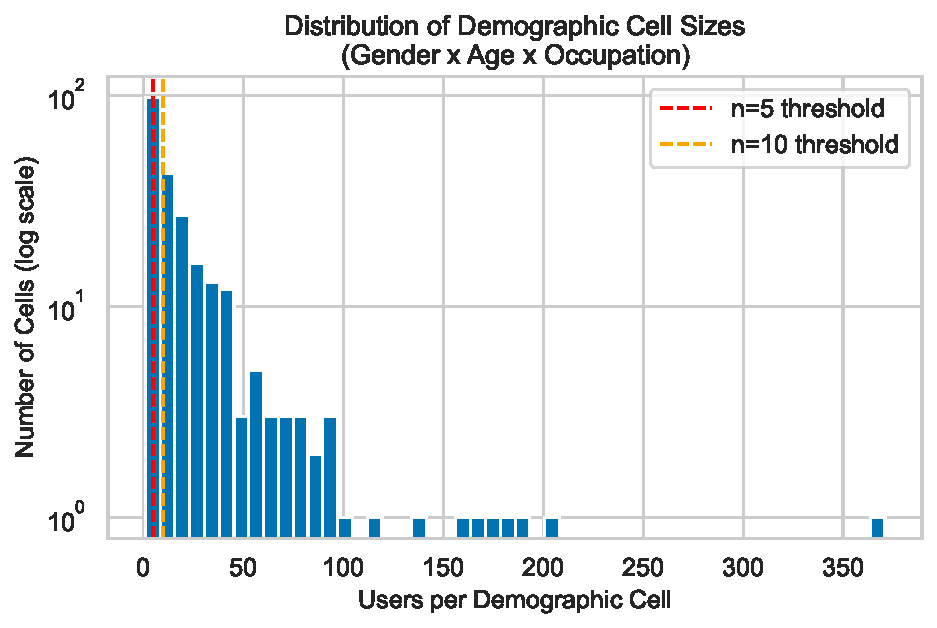
\includegraphics[width=0.65\columnwidth]{images/ml1m_cell_size_distribution.pdf}
    \caption{Distribution of demographic cell sizes (Gender$\times$Age$\times$Occupation). Red and orange lines mark the $n=5$ and $n=10$ thresholds.}
    \label{fig:app-cell-dist}
\end{figure}


\subsubsection{Per-User Rating Activity}

Figure~\ref{fig:app-per-user} shows the per-user rating count distribution.
The distribution is heavily right-skewed: the median user has rated 96 movies, but the mean is 166 due to a long tail of power raters (max 2{,}314).
Every user has at least 20 ratings, as guaranteed by the ML-1M inclusion criterion.

With a 20\% temporal split, every user contributes at least 4 test items (mean 32.7, median 19), and the train/test split yields 802{,}553 / 197{,}656 ratings.

\begin{figure}[h]
    \centering
    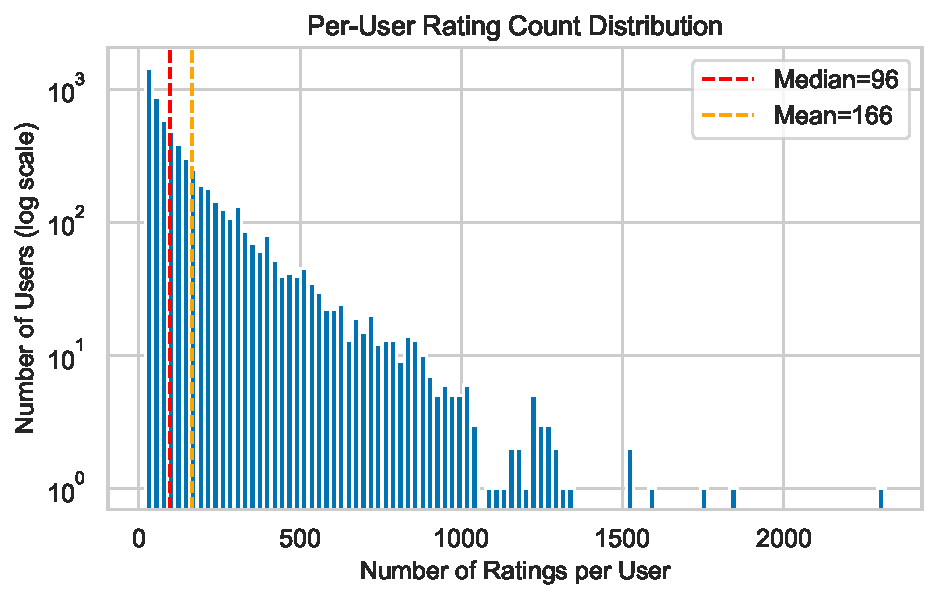
\includegraphics[width=0.65\columnwidth]{images/ml1m_per_user_ratings.pdf}
    \caption{Per-user rating count distribution (log-scale y-axis). Red: median (96); orange: mean (166).}
    \label{fig:app-per-user}
\end{figure}


\subsubsection{Temporal Distribution}

Figure~\ref{fig:app-temporal} shows the monthly rating volume.
Activity is concentrated in the first year (April--December 2000), with a gradual decline through 2001--2003.
This non-uniform temporal distribution means the chronological test split (last 20\% per user) will contain later-rated movies, which may differ systematically in genre from earlier ratings.

\begin{figure}[h]
    \centering
    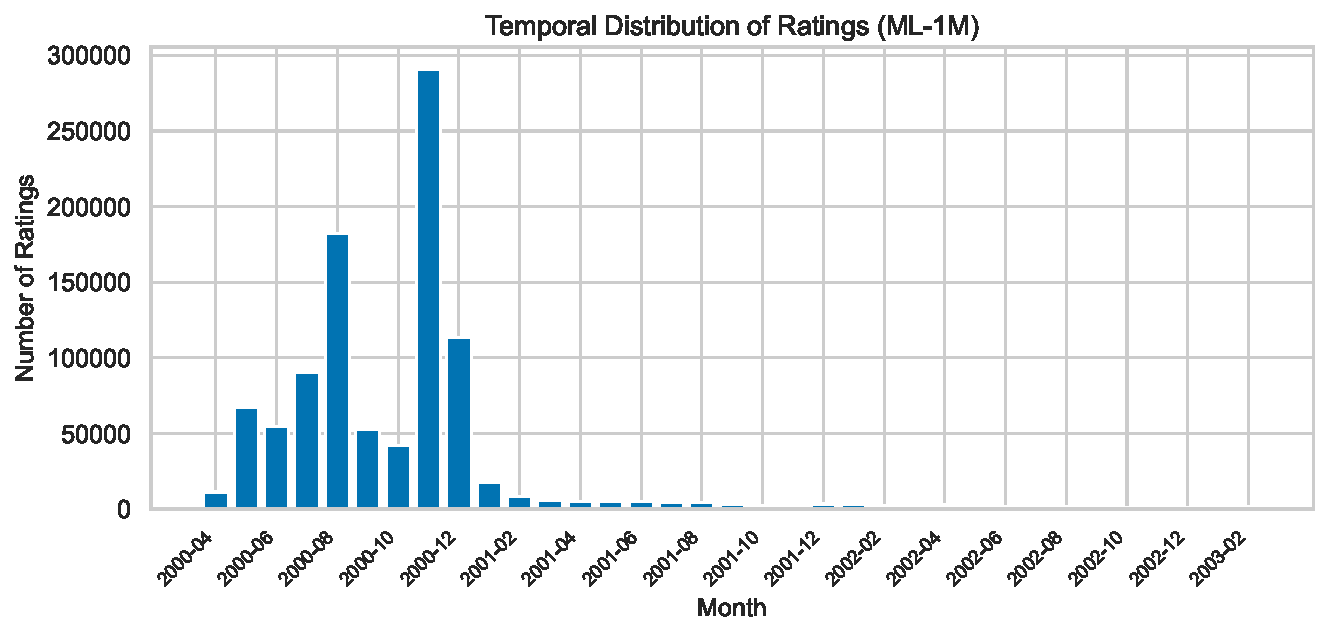
\includegraphics[width=0.8\columnwidth]{images/ml1m_temporal_distribution.pdf}
    \caption{Monthly rating volume in ML-1M (April 2000 to February 2003).}
    \label{fig:app-temporal}
\end{figure}


\subsubsection{Popularity Bias}

The ML-1M movie popularity distribution exhibits a strong long tail (Figure~\ref{fig:app-popularity}):
\begin{itemize}
    \item \textbf{Gini coefficient:} 0.634
    \item The top 20\% of movies (741 films) account for 65.2\% of all ratings.
    \item 446 movies (12.0\%) have fewer than 10 ratings; 1{,}192 (32.2\%) have fewer than 50.
    \item Only 207 movies (5.6\%) exceed 1{,}000 ratings.
\end{itemize}

The 10 most-rated movies are: \emph{American Beauty} (3{,}428), \emph{Star Wars: Episode IV} (2{,}991), \emph{Star Wars: Episode V} (2{,}990), \emph{Star Wars: Episode VI} (2{,}883), \emph{Jurassic Park} (2{,}672), \emph{Saving Private Ryan} (2{,}653), \emph{Terminator 2} (2{,}649), \emph{The Matrix} (2{,}590), \emph{Back to the Future} (2{,}583), \emph{Silence of the Lambs} (2{,}578).

Figure~\ref{fig:app-rating-by-pop} shows that popular movies receive slightly higher mean ratings (mean 3.7 for top quintile vs.\ 3.4 for bottom quintile) but also have lower rating variance, suggesting more consensus on well-known films and more polarization on niche titles.

\begin{figure}[h]
    \centering
    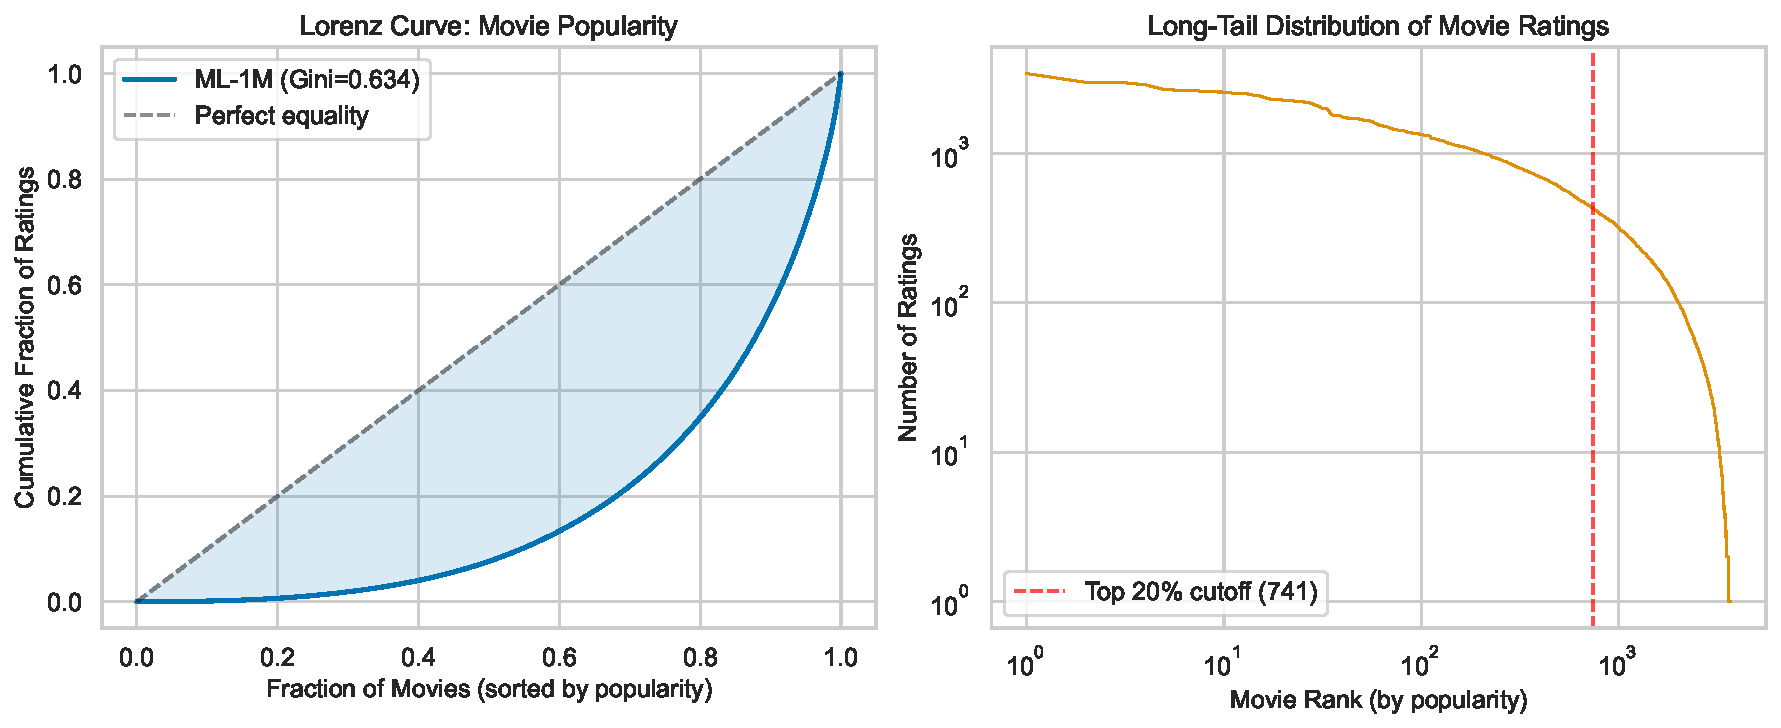
\includegraphics[width=\textwidth]{images/ml1m_popularity_bias.pdf}
    \caption{\textbf{Left:} Lorenz curve for movie popularity (Gini = 0.634). \textbf{Right:} Long-tail distribution on log-log scale.}
    \label{fig:app-popularity}
\end{figure}

\begin{figure}[h]
    \centering
    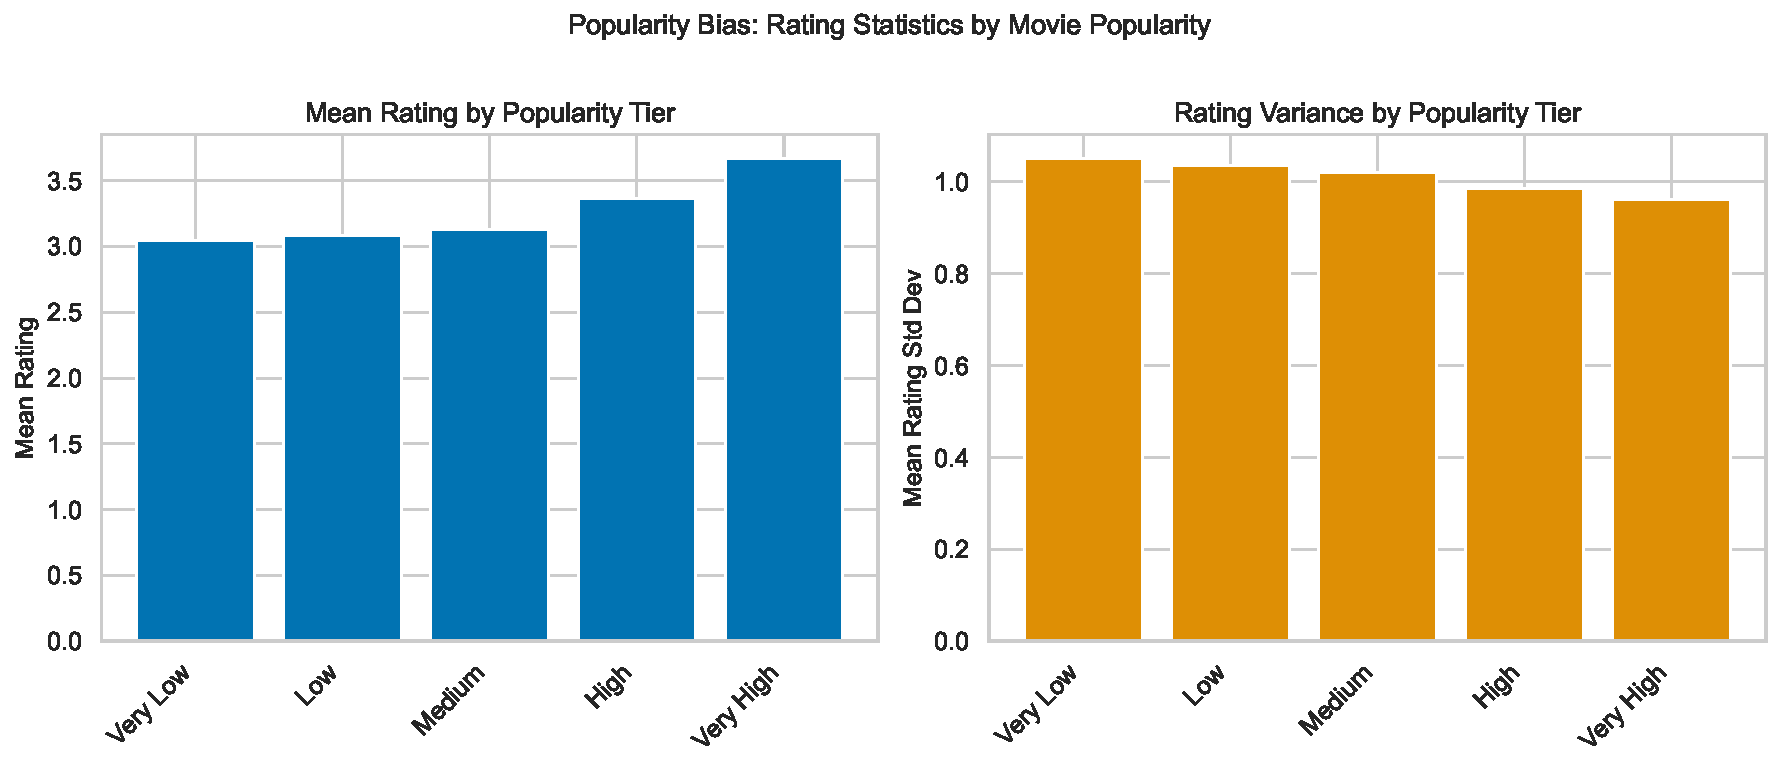
\includegraphics[width=\textwidth]{images/ml1m_rating_by_popularity.pdf}
    \caption{Mean rating and rating standard deviation stratified by movie popularity quintile.}
    \label{fig:app-rating-by-pop}
\end{figure}


\subsubsection{Genre Analysis}

ML-1M movies span 18 genres (many movies have multiple genres).
Drama (1{,}603 movies) and Comedy (1{,}200) are the most common; Film-Noir (44) and Western (68) are the rarest.

\paragraph{Genre preferences by gender.}
Figure~\ref{fig:app-genre-gender} shows the mean rating difference (Male $-$ Female) per genre.
Females rate Romance ($+$0.13) and Musical ($+$0.09) higher; males rate Sci-Fi ($+$0.10), Horror ($+$0.08), and Film-Noir ($+$0.07) higher.
These differences are statistically significant but small in magnitude.

\paragraph{Genre preferences by age.}
Figure~\ref{fig:app-genre-age} shows the mean rating by genre and age group.
Older users (56+) give consistently higher ratings across most genres (mean 3.76 vs.\ 3.42 for Under~18).
The largest age-driven genre gap is in Film-Noir (3.96 for 56+ vs.\ 3.21 for Under~18) and War (4.01 for 56+ vs.\ 3.44 for Under~18).
Younger users rate Animation and Children's genres relatively higher.

\paragraph{Genre co-occurrence.}
Figure~\ref{fig:app-genre-cooccurrence} shows the genre co-occurrence matrix.
The strongest co-occurrence is Action--Adventure (160 movies), followed by Comedy--Romance (148) and Action--Thriller (130).

\begin{figure}[h]
    \centering
    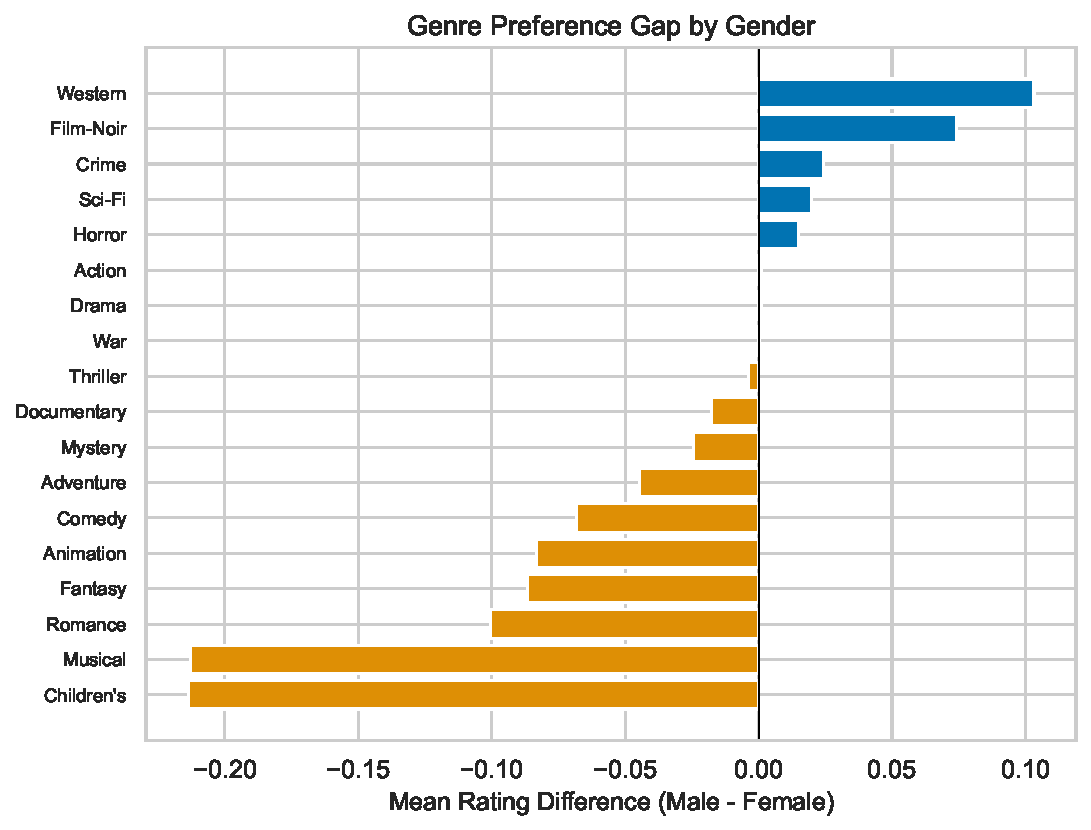
\includegraphics[width=0.65\columnwidth]{images/ml1m_genre_gender_gap.pdf}
    \caption{Mean rating gap by genre (Male $-$ Female). Positive values indicate genres preferred by males.}
    \label{fig:app-genre-gender}
\end{figure}

\begin{figure}[h]
    \centering
    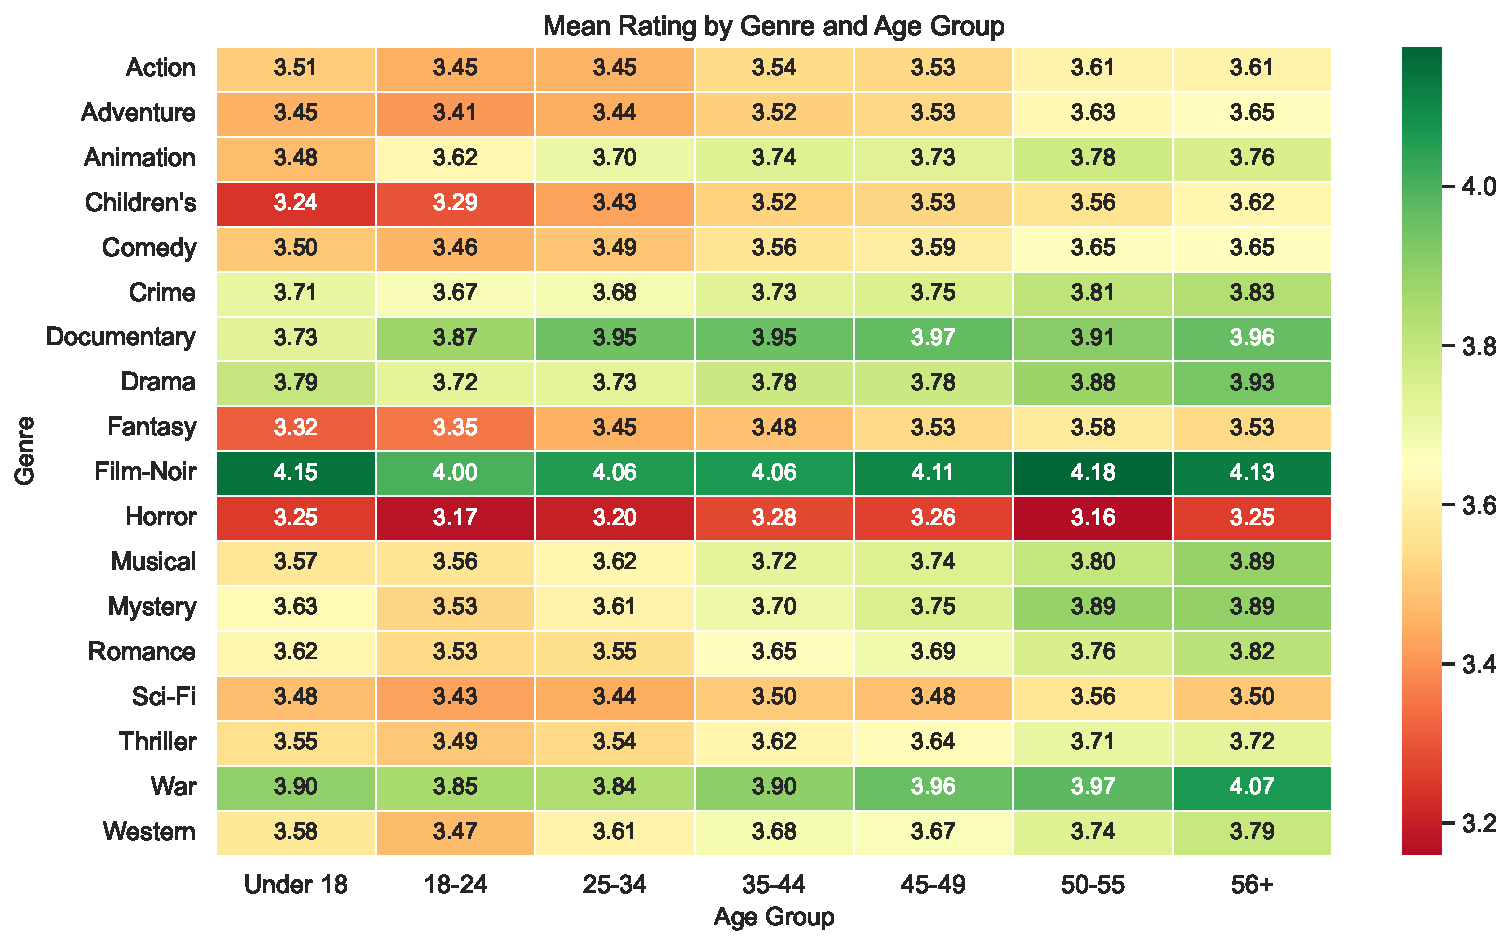
\includegraphics[width=\textwidth]{images/ml1m_genre_age_heatmap.pdf}
    \caption{Mean rating by genre and age group. Older users give higher ratings overall; the largest age-driven gap is in Film-Noir and War.}
    \label{fig:app-genre-age}
\end{figure}

\begin{figure}[h]
    \centering
    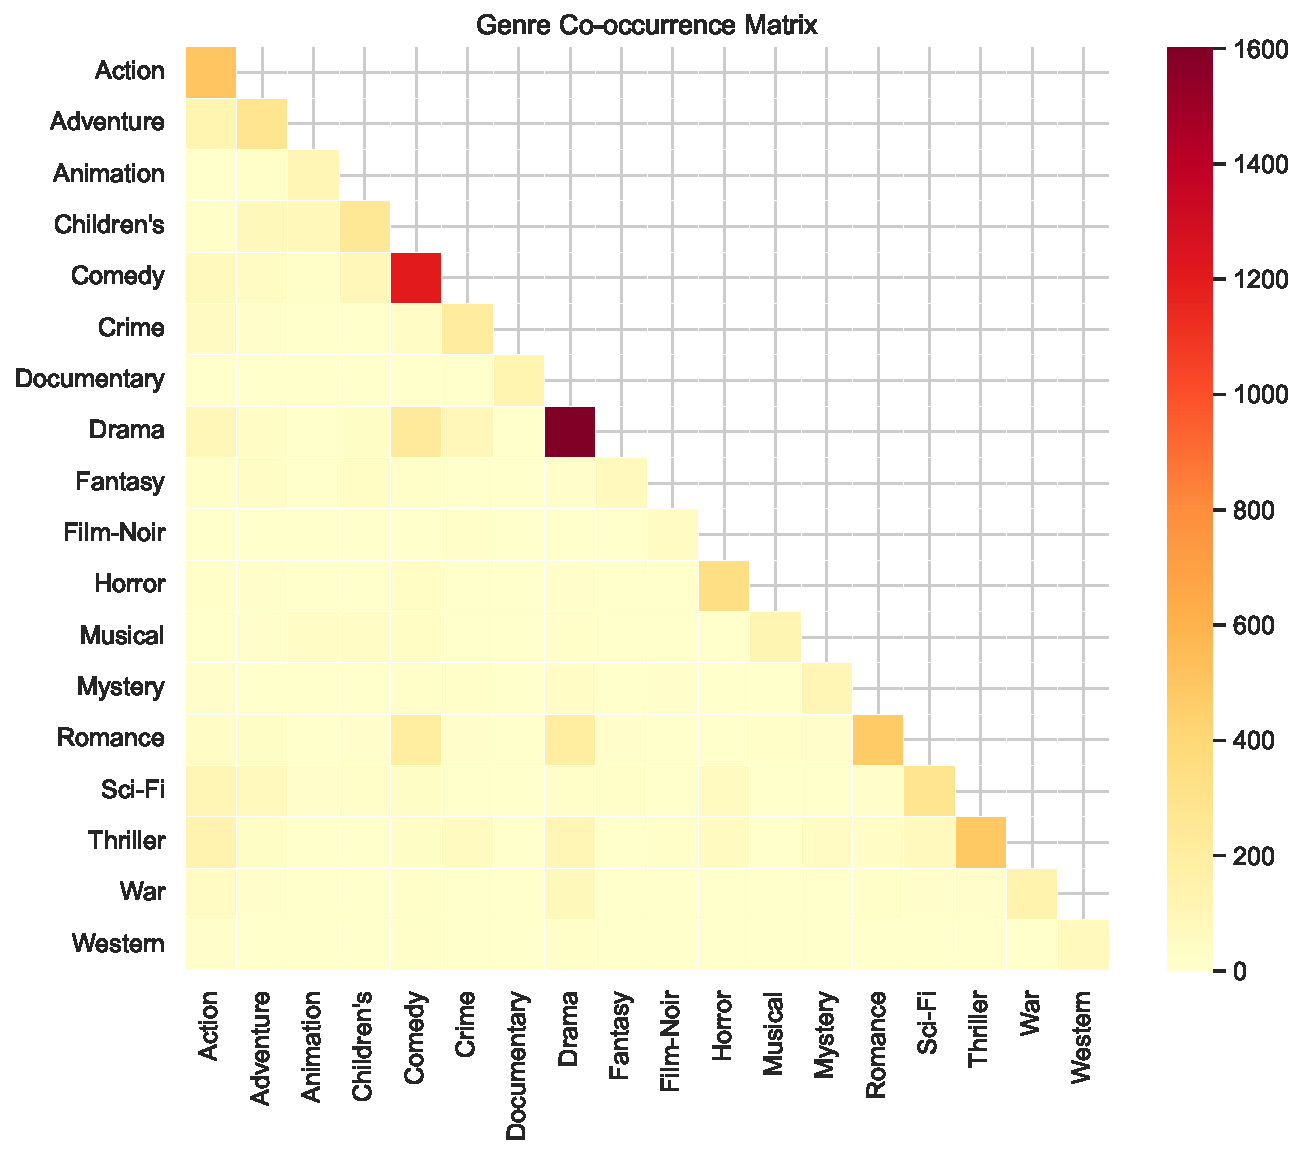
\includegraphics[width=0.65\columnwidth]{images/ml1m_genre_cooccurrence.pdf}
    \caption{Genre co-occurrence matrix (lower triangle). Strongest: Action--Adventure (160), Comedy--Romance (148).}
    \label{fig:app-genre-cooccurrence}
\end{figure}


\subsubsection{Within- vs.\ Between-Demographic Variance}
\label{app:variance-decomposition}

A key question for persona-conditioned simulation is whether demographics predict meaningful variance in ratings.
Table~\ref{tab:variance} reports the $\eta^2$ (ratio of between-group to total sum of squares) for each demographic axis.

\begin{table}[h]
\centering
\caption{Variance decomposition: fraction of total rating variance explained by demographic grouping ($\eta^2$).}
\label{tab:variance}
\small
\begin{tabular}{@{}lr@{}}
\toprule
\textbf{Grouping} & \textbf{$\eta^2$ (\%)} \\
\midrule
Gender & 0.039 \\
Age & 0.376 \\
Occupation & 0.268 \\
Gender $\times$ Age & 0.477 \\
Gender $\times$ Age $\times$ Occupation & 1.562 \\
\bottomrule
\end{tabular}
\end{table}

Even the most granular demographic grouping (full three-way cell) explains only 1.56\% of total rating variance.
This confirms that \emph{within-demographic variance overwhelmingly dominates}: two users in the same Gender$\times$Age$\times$Occupation cell can have drastically different movie preferences.
This finding directly motivates persona-level (rather than purely demographic-level) simulation and suggests that the key evaluation signal is within-cell differentiation---the ability of richer personas to capture individual taste variation that demographics miss.

\begin{figure}[h]
    \centering
    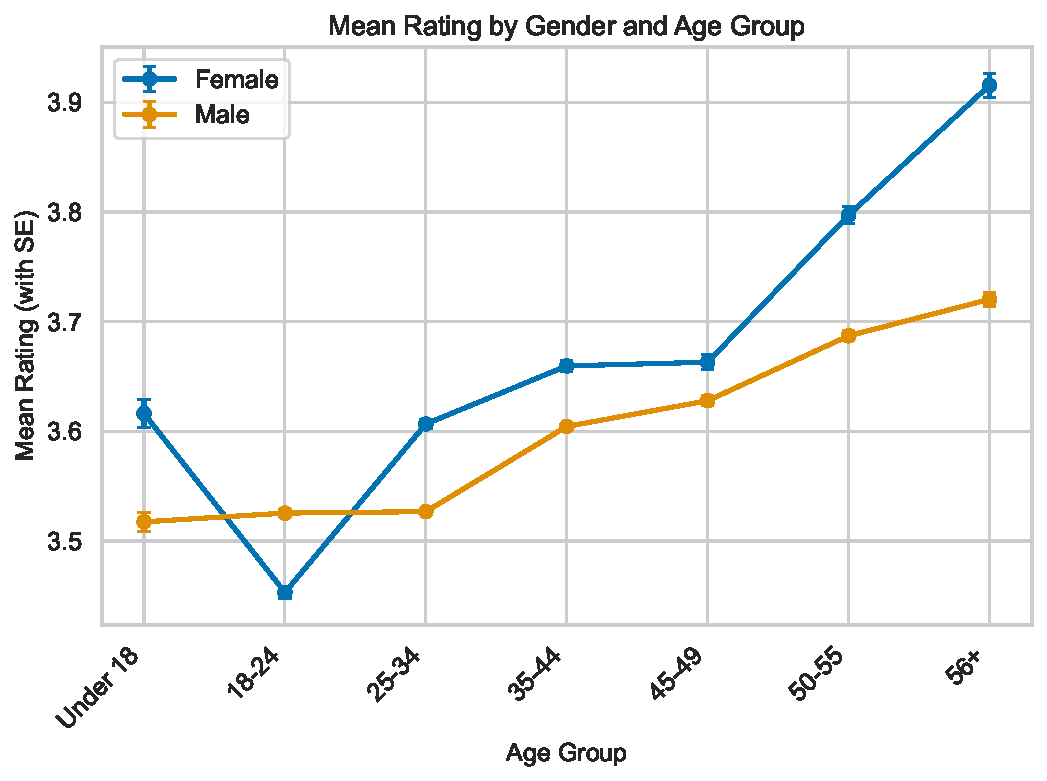
\includegraphics[width=0.65\columnwidth]{images/ml1m_mean_rating_by_demographic.pdf}
    \caption{Mean rating by Gender$\times$Age with standard error bars. Between-group differences are statistically significant but small (0.2--0.3 stars). Older users and female users rate slightly higher on average.}
    \label{fig:app-mean-rating-demo}
\end{figure}


\subsubsection{Temporal Split Validation}

With the proposed $p=20\%$ chronological split:
\begin{itemize}
    \item \textbf{Train set:} 802{,}553 ratings
    \item \textbf{Test set:} 197{,}656 ratings
    \item Every user contributes at least 4 test items (mean 32.7, median 19).
    \item 100\% of users have $\geq$4 test items, supporting per-user NDCG computation.
\end{itemize}

\subsubsection{Summary of EDA Findings}

\begin{enumerate}
    \item ML-1M is integrity-verified: zero orphan records, all documented schema constraints hold.
    \item The user base skews male (72\%), young (53\% aged 18--34), and tech-oriented (top occupations: student, executive, educator, engineer, programmer).
    \item Demographics explain $<$2\% of rating variance ($\eta^2 = 0.016$ for the full three-way cell). Within-demographic taste variation dominates.
    \item Popularity bias is substantial (Gini 0.634); evaluation must include popularity-debiased metrics.
    \item Gender$\times$Age provides 14 well-populated cells (min 78 users) suitable as the primary stratification. The full three-way stratification is too sparse for reliable subgroup evaluation.
    \item Genre preferences vary systematically with demographics (age more than gender), providing signal that persona-conditioned simulation should exploit.
    \item The 20\% temporal split yields a clean train/test partition with sufficient per-user test items for individual-level evaluation.
\end{enumerate}
